\def\difficulty{2}
\sujet{Introduction to wavelets}
\index{Wavelets!Definition}
\index{Fourier Transform}

\begin{note}This tutorial introduces practically the basic wavelet decomposition and reconstruction algorithms. The objectives are to code some basic programs that will decompose and reconstruct 1D and 2D signals.\end{note}

\section{Introduction}
Wavelets are based on a mother wavelet $\Psi$ ($s$ is a scale parameter, $\tau$ is the time translation factor $(s,\tau)\in \R^*_+ \times 
\R$):
$$\forall t \in \R, \psi_{s,\tau}(t) = \frac{1}{\sqrt{s}}\Psi\left( \frac{t-\tau}{s}\right) $$

The continuous wavelet transform is written as follows, where $\psi^*$ means the complex conjugate of $\psi$ and $<.,.>$ is the complex scalar 
product (Hermitian form):
$$g(s,\tau)=\int_{-\infty}^\infty f(t)\psi^*_{s,\tau}(t)\textrm{d}s\textrm{d}\tau =<f,\psi_{s,\tau}>$$

The reconstruction is defined by:
$$f(t) = \frac{1}{C} \int_{-\infty}^{\infty} \int_{-\infty}^{\infty} \frac{1}{|s|^2} g(s,\tau) \psi_{s,\tau}(t) \textrm{d} s \; 
\textrm{d}\tau$$
with $$C= \int_{-\infty}^{\infty} \frac{|\hat{\Psi}(\omega)|^2}{|\omega|} \textrm{d}\omega $$
and $\hat{\Psi}$ is the Fourier Transform of $\Psi$.

The discrete wavelet transform corresponds to a sampling of the scales. To compute the different scales, one has to introduce a ``father'' 
wavelet, that similarly defines a family of functions orthogonal to the family $\psi_{s,\tau}$.

\section{Fast discrete wavelet decomposition / reconstruction}
A simple algorithm (cascade algorithm, from Mallat) is defined as two convolutions (by a lowpass $ld$ filter for the projection on the 
$\psi$ family, and a high pass $hd$ filter for the orthogonal projection) followed by a subsampling (see Fig. 
\ref{fig:wavelets:decomposition}).

\begin{figure}[H]
 \centering
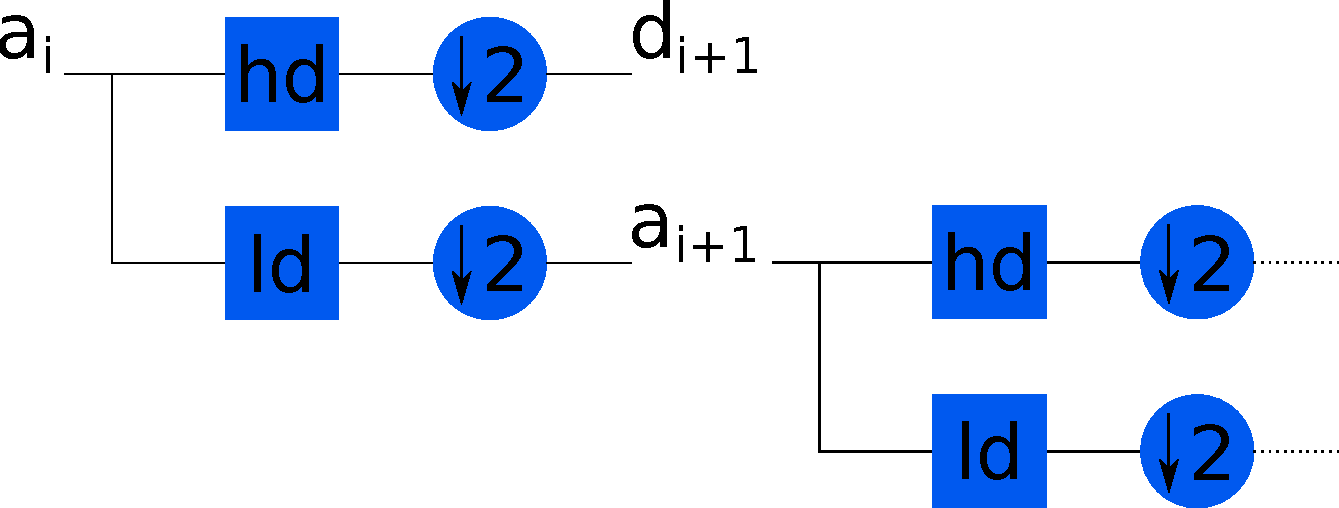
\includegraphics[width=7cm]{schema_decomposition}
\caption{\textls[-20]{Algorithm for wavelet decomposition. First, a convolution is performed (square node), then, a subsampling. $a_i$ stands for 
decomposition at scale i, $d_i$ stands for detail at scale i.}}
\label{fig:wavelets:decomposition}
\end{figure}

\subsection{Simple 1D example}
Let's consider the signal $[ 4; 8; 2; 3; 5; 18; 19; 20]$. We will use the Haar wavelets defined by $ld=[1; 1]$ and $hd=[-1;1]$. Basically, 
these filters perform a mean and a difference (see Table \ref{tab:wavelets:decomposition}). The result of the decomposition in 3 scales with 
these wavelets is the concatenation of the details and the final approximation 
$$C=\{[-4    ;-1  ; -13  ;  -1]; [7 ;  -16]; [-45]; [ 79] \}$$

\begin{mcomment}
\begin{mremark}
For the sake of simplicity, it is recommended to use the structure \minline{cell} of \matlabregistered{} to store the decomposition of all detail 
vectors as well as the final approximation vector.
\end{mremark}
\end{mcomment}

\begin{table}[H]
\begin{center}
\begin{tabular}{|c|c|c|}
\hline
Scale $i$& Approximation $a_i$ & Details $d_i$\\ \hline
0 (original signal)&  $[ 4; 8; 2; 3; 5; 18; 19; 20]$& \\
1& $[12 ;    5 ;   23 ;   39 ]$& $[-4;-1;-13;-1]$\\
2 & $[17; 62]$ & $[7 ;-16]$\\
3 & $[79]$& $[-45]$\\
\hline
\end{tabular}
\end{center}
\caption{Illustration of Haar decomposition in a simple signal.\label{tab:wavelets:decomposition}}
\end{table}

\begin{qbox}
In the case of these Haar wavelets, code a function that performs the decomposition for a given number of scales. The prototype of this 
function will be:

\begin{mcomment}
\begin{matlab} 
function C=simpleWaveDec(signal1D, nb_scales)
% wavelet decomposition of <signal1D> into <nb_scales> scales
\end{matlab}
\end{mcomment}


\begin{pcomment}
\begin{python}
def simpleWaveDec(signal, nb_scales):
    """
    wavelet decomposition of <signal> into <nb_scales> scales
    This function uses Haar wavelets for demonstration purposes.
    """
\end{python}
\end{pcomment}

\end{qbox}

\subsection{Reconstruction}
To reconstruct the original signal (see Fig. \ref{fig:wavelets:reconstruction}), we need the definition of two reconstruction filters, $hr$ 
and $lr$. For the sake of simplicity, we use $lr=ld/2$ and $hr=-hd/2$. These filter will perform an exact reconstruction of our original 
signal.

\begin{figure}[H]
 \centering\caption{Reconstruction algorithm. The oversampling is done by inserting zeros.}
 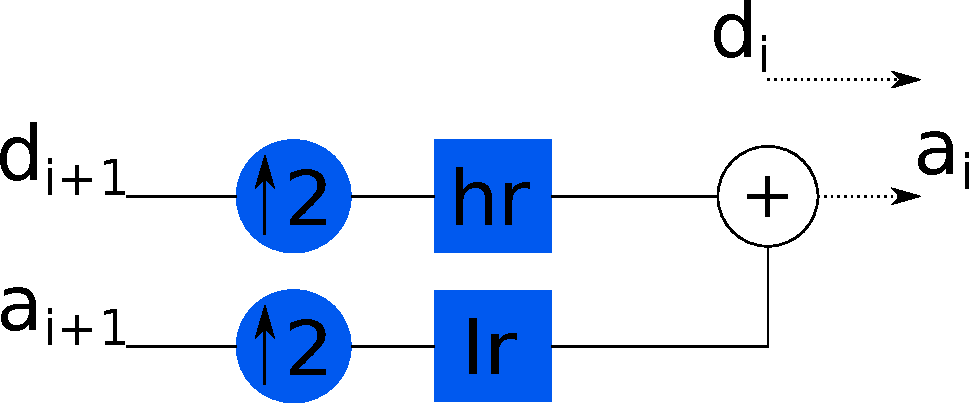
\includegraphics[width=7cm]{schema_reconstruction.pdf}%
 \label{fig:wavelets:reconstruction}%
\end{figure}

Using this algorithm, you can now go on to the next exercise.

%\section{Simple 1D reconstruction}
\begin{qbox}
Code a function that performs the reconstruction of the signal. The prototype of this function will be, with the previous definition of C:
\begin{mcomment}
\begin{matlab} 
function signal=simpleWaveRec(C)
% wavelet simple reconstruction function of a 1D signal
% C: Wavelet coefficients in cell of arrays
% signal: reconstructed signal
\end{matlab}
\end{mcomment}

\begin{pcomment}
\begin{python}
def simpleWaveRec(C):    
    """
    wavelet simple reconstruction function of a 1D signal
    C: Wavelet coefficients 
    """
\end{python}
\end{pcomment}
\end{qbox}

\section{2D wavelet decomposition}
Let $A$ be the matrix of an image. We consider that $A$ is of size $2^n\times 2^n$, $n\in\mathbb{N}$. We consider, as for the 1D transform, 
the filters $ld$ and $hd$.

The wavelet decomposition is as follows:
\begin{itemize}
 \item Apply $ld$ and $hd$ on rows of A. Results are denoted $ld_r A$ and $hd_r A$, of size $2^n\times 2^{n-1}$, with $r$ standing for row.
 \item Then, apply $ld$ and $hd$ again, to get the four new matrices: $ld_c ld_r A$, $ld_c hd_r A$, $hd_c ld_r A$ and $hd_c hd_r A$, of 
sizes $2^{n-1}\times 2^{n-1}$, with $c$ standing for column. The matrix $ld_c ld_r A$ is the approximation, and the other matrices are the 
details.
\end{itemize}

\begin{qbox}
\begin{itemize} \item Code a function to perform the wavelet decomposition and for a given number of scales (lower than $n$). Test 
it on images of size $2^n\times 2^n$.
 \item Code the reconstruction function.
\end{itemize}

\end{qbox}


\section{Built-in functions}
Let us explore some built-in functions. 

\subsection{Continuous wavelet decomposition}
One has to make the difference between the continuous wavelet transform and the discrete transform.

\begin{mcomment}
\begin{mremark}
The \matlabregistered{} function that performs continuous wavelet transform is \minline{cwt}.
 A GUI dedicated to wavelets is available in \matlabregistered{}: type the command \minline{wavemenu} and try some 1D and 2D signals. 
\begin{matlab}
load noissin; % load a signal1D

% perform continuous wavelet transform at scales specified by
% 1:48
c = cwt(noissin, 1:48, 'db4', 'plot');
\end{matlab}
\end{mremark}
\end{mcomment}

\begin{phelp}
In \pinline{scipy.signal} you can find function to perform wavelets decomposition, and among them \pinline{cwt} for the continuous wavelet transform. There is also the module \pinline{pywt} that may be more developped (see also \pinline{cwt}).
\end{phelp}

\begin{figure}[H]
 \centering\caption{Continuous wavelet transform.}%
 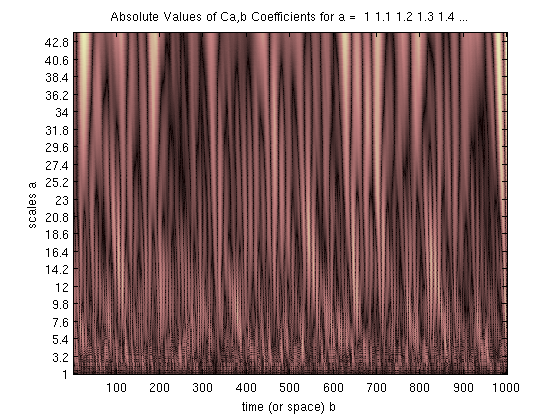
\includegraphics[width=10cm]{cwt.png}%
\end{figure}

\subsection{Discrete decomposition}

\begin{qbox}
 \begin{enumerate}
  \item Generate the signal $\sin(2\pi * f_1*t)+ \sin(2\pi*f_2*t)$, with $f_1=3$Hz and $f_2=50$Hz.
  \item Apply the wavelet transformation for a given wavelet (like 'db4'). 
  \item Display the 5th approximation of the wavelet decomposition.
  \item Display the 4th detail coefficients of the wavelet decomposition.
 \end{enumerate}
\end{qbox}

\begin{mcomment}
\begin{mremark}
Each of the \matlabregistered{} function is available for 1D, 2D or even 3D signals. You can test the following functions \minline{wavedec}, 
\minline{wavedec2} or \minline{wavedec3}:
\begin{matlab}
[C,L] = wavedec(signal, scale, 'wavelet_name')
[C,L] = wavedec(signal, scale, ld, hd)
\end{matlab}
\end{mremark}
\end{mcomment}
\begin{pcomment}
\begin{premark}
Look at \pinline{pywt.downcoef} for the decomposition at a given level and \pinline{pywt.wavedec} for the entire decomposition.
\end{premark}
\end{pcomment}
